\section{MongoDB}

\subsection{Criação da base de dados}

\subsubsection{Motivação}

Por esta ser uma base de dados orientada a documentos, tem várias vantagens face ao MySQL, para além de ser escalável horizontalmente, é mais facil de manter, atualizar e é ótima para coletar informações referentes a um objeto, evitando joins de tabelas usados pelo MySQL visto este ter toda a informação de um objeto num mesmo documento.

\subsubsection{Criação - modificações}

Pra a criação desta base de dados supusemos ser uma aplicação da loja na qual só se pretende obter informações sobre que utilizador consome filmes em que loja quem o atendeu, em que data e qual o preço. Para além disso é importante saber as carateristicas dos filmes presentes nas lojas, as linguas em que estão, quais os atores que participaram e as categorias em que se insere.

\subsection{Criação - Estrutura da Base de Dados}

\par Em seguida apresentam-se os documentos gerados com base nos requisitos para a base de dados MongoDB.\newline
\begin{itemize}
\item Filme:  {"id": , "title": , "release\_year": , "descrição": , "original\_language": , "foreign\_language": , "categorys": , "actors": }\newline

\item Pagamento: {"store\_id": , "customer": , "date": , "amount": , "staff": }
\end{itemize}

\subsection{Preenchimento da Base de Dados}

\begin{itemize}
\item \textbf{firstQuery = "SELECT f.title,f.release\_year,f.description,c.name AS Category,a.first\_name,a.last\_name, language.name AS Foreign\_language,extra.name AS Original\_language,f.film\_id FROM film AS f} 
\par \textbf{LEFT JOIN film\_category AS fc ON fc.film\_id = f.film\_id }
\par \textbf{LEFT JOIN category AS c ON c.category\_id = fc.category\_id }
\par \textbf{LEFT JOIN film\_actor AS fa ON fa.film\_id = f.film\_id }
\par \textbf{LEFT JOIN actor AS a ON a.actor\_id = fa.actor\_id }
\par \textbf{LEFT JOIN language ON language.language\_id = f.language\_id} 
\par \textbf{LEFT JOIN ( SELECT f.film\_id,l.name FROM film AS f 
               LEFT JOIN language AS l ON l.language\_id = f.original\_language\_id 
               WHERE f.original\_language\_id is not null) 
           extra ON f.film\_id = extra.film\_id"}\newline

\item \textbf{mycursor.execute(firstQuery)}\newline
\item \textbf{filmRecords = mycursor.fetchall()}\newline
\item \textbf{myFilmIt = iter(filmRecords)}\newline

\par Em seguida podemos observar o loop usado para criar os documentos film.\newline
\begin{figure}[H]

  \centering

  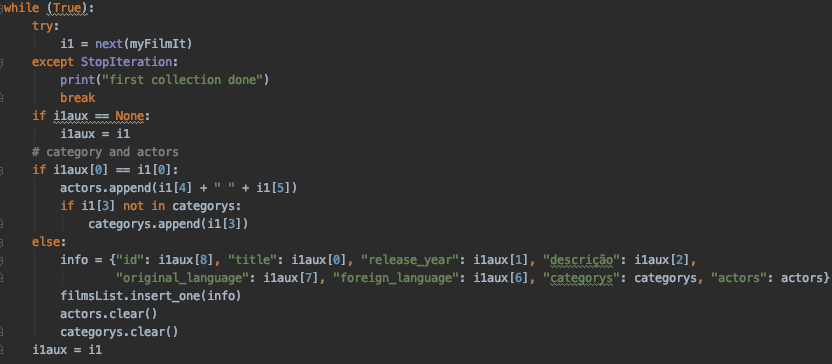
\includegraphics[scale = 0.45]{ciclo.png}

  \caption {Ciclo que gera cada documento Film guardado na base de dados MongoDB}

  \label {fig1}

\end{figure}

Cada objeto iterado neste ciclo while corresponde a um film, podendo haver filmes repetidos em iterações sucessivas cuja única diferença reside sempre no ator e pode ter também diferentes categorias, tendo portanto, cada iteração, um ator diferente e uma ou nenhuma categoria. Assim fazendo uso do ciclo com a verificação do id de cada filme sendo igual permite que identifiquemos o mesmo filme em várias iterações e possamos adicionar os atores todos numa string bem como as categorias. Quando a verificação da igualdade do filme falha sabemos que podemos adicionar o filme á base de dados pois já coletámos todos os atores e categorias deste.

\end{itemize}
\subsection{Querys a Base de Dados}

Em seguida listam-se algumas das querys feitas á base de dados Mongo e as respetivas respostas.

\begin{itemize}
\item \textbf{filmsList.find({}, {"title": 1, "original\_language": 1, "foreign\_language": 1, "\_id": 0})}

\item 
\begin{figure}[H]

  \centering

  \hbox{\hspace{-11.5em} 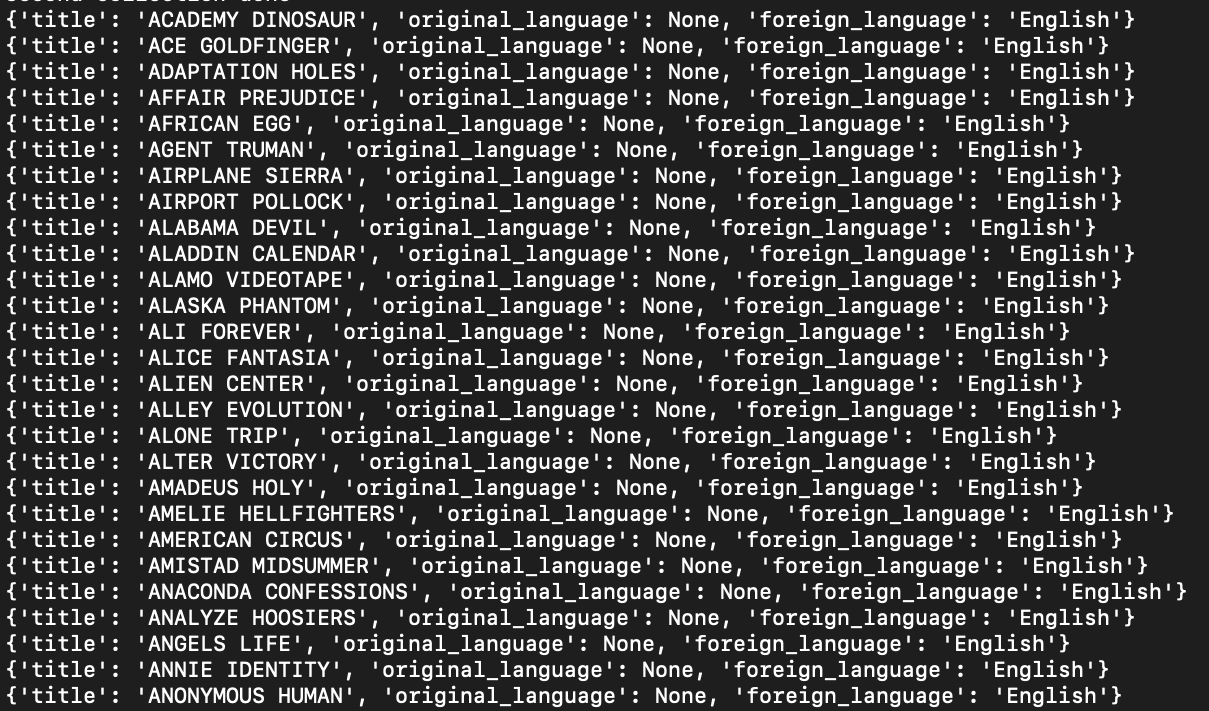
\includegraphics[scale = 0.45]{mongoQuery1.png}}

  \caption {Excerto do resultado da primeira query feita á base de dados MongoDB}

  \label {fig2}

\end{figure}

\item \textbf{query2Mongo = filmsList.find({"title": 'ACADEMY DINOSAUR'}, {"title": 1, "actors": 1, "\_id": 0})}

\begin{figure}[H]

  \centering

  \hbox{\hspace{-11.5em} 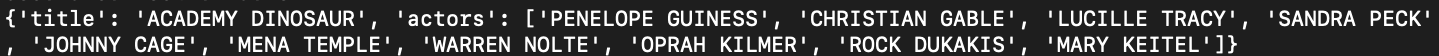
\includegraphics[scale = 0.40]{mongoQuery2.png}}

  \caption {Resultado da segunda query feita á base de dados MongoDB}

  \label {fig3}

\end{figure}

\item \textbf{query3Mongo = paymentList.find({'customer': 'AUSTIN CINTRON'}, { "\_id": 0})}

\begin{figure}[H]

  \centering

  \hbox{\hspace{-11.5em} 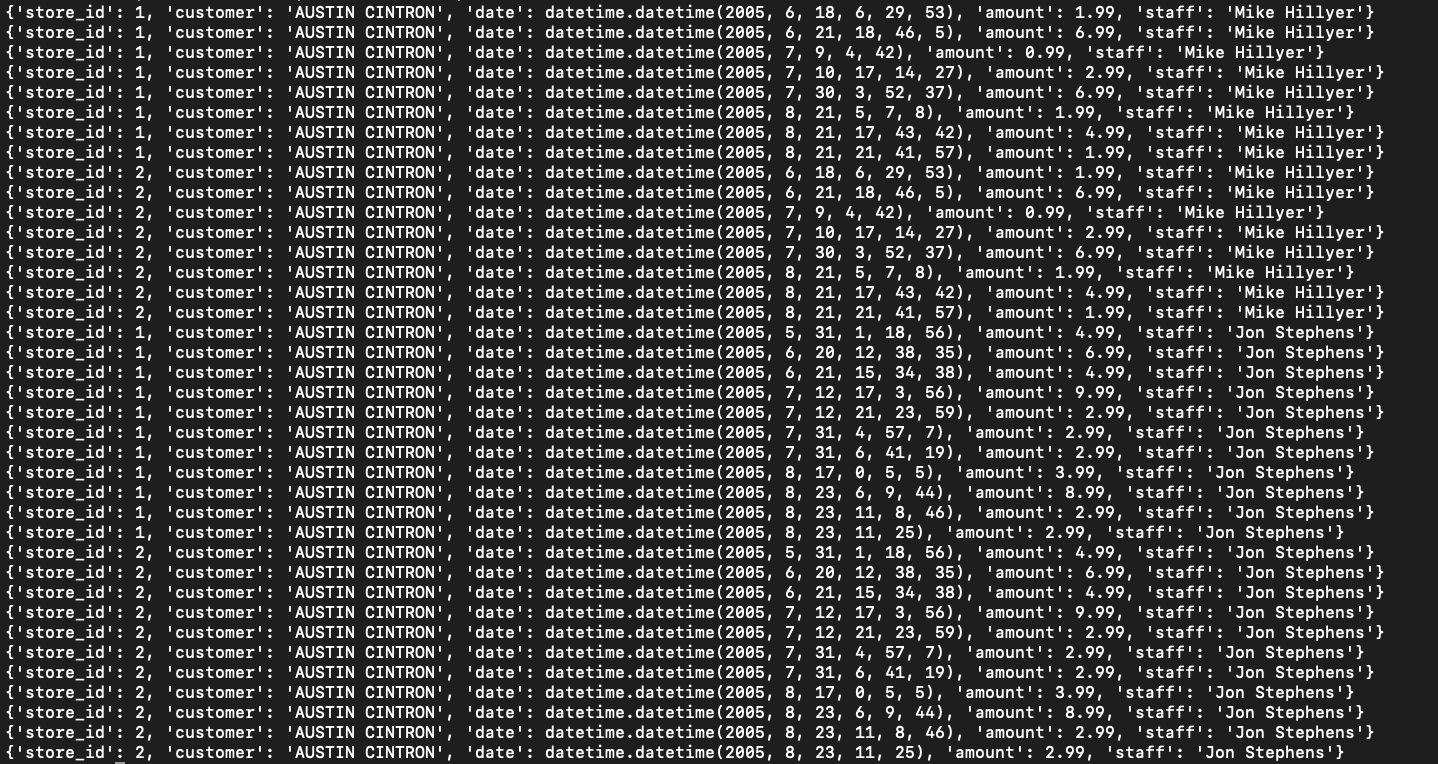
\includegraphics[scale = 0.40]{mongoQuery3.png}}

  \caption {Resultado da terceira query feita á base de dados MongoDB}

  \label {fig4}

\end{figure}
\end{itemize}



